% Options for packages loaded elsewhere
\PassOptionsToPackage{unicode}{hyperref}
\PassOptionsToPackage{hyphens}{url}
%
\documentclass[
  ignorenonframetext,
]{beamer}
\usepackage{pgfpages}
\setbeamertemplate{caption}[numbered]
\setbeamertemplate{caption label separator}{: }
\setbeamercolor{caption name}{fg=normal text.fg}
\beamertemplatenavigationsymbolsempty
% Prevent slide breaks in the middle of a paragraph
\widowpenalties 1 10000
\raggedbottom
\setbeamertemplate{part page}{
  \centering
  \begin{beamercolorbox}[sep=16pt,center]{part title}
    \usebeamerfont{part title}\insertpart\par
  \end{beamercolorbox}
}
\setbeamertemplate{section page}{
  \centering
  \begin{beamercolorbox}[sep=12pt,center]{part title}
    \usebeamerfont{section title}\insertsection\par
  \end{beamercolorbox}
}
\setbeamertemplate{subsection page}{
  \centering
  \begin{beamercolorbox}[sep=8pt,center]{part title}
    \usebeamerfont{subsection title}\insertsubsection\par
  \end{beamercolorbox}
}
\AtBeginPart{
  \frame{\partpage}
}
\AtBeginSection{
  \ifbibliography
  \else
    \frame{\sectionpage}
  \fi
}
\AtBeginSubsection{
  \frame{\subsectionpage}
}

\usepackage{amsmath,amssymb}
\usepackage{iftex}
\ifPDFTeX
  \usepackage[T1]{fontenc}
  \usepackage[utf8]{inputenc}
  \usepackage{textcomp} % provide euro and other symbols
\else % if luatex or xetex
  \usepackage{unicode-math}
  \defaultfontfeatures{Scale=MatchLowercase}
  \defaultfontfeatures[\rmfamily]{Ligatures=TeX,Scale=1}
\fi
\usepackage{lmodern}
\ifPDFTeX\else  
    % xetex/luatex font selection
\fi
% Use upquote if available, for straight quotes in verbatim environments
\IfFileExists{upquote.sty}{\usepackage{upquote}}{}
\IfFileExists{microtype.sty}{% use microtype if available
  \usepackage[]{microtype}
  \UseMicrotypeSet[protrusion]{basicmath} % disable protrusion for tt fonts
}{}
\makeatletter
\@ifundefined{KOMAClassName}{% if non-KOMA class
  \IfFileExists{parskip.sty}{%
    \usepackage{parskip}
  }{% else
    \setlength{\parindent}{0pt}
    \setlength{\parskip}{6pt plus 2pt minus 1pt}}
}{% if KOMA class
  \KOMAoptions{parskip=half}}
\makeatother
\usepackage{xcolor}
\newif\ifbibliography
\setlength{\emergencystretch}{3em} % prevent overfull lines
\setcounter{secnumdepth}{-\maxdimen} % remove section numbering

\usepackage{color}
\usepackage{fancyvrb}
\newcommand{\VerbBar}{|}
\newcommand{\VERB}{\Verb[commandchars=\\\{\}]}
\DefineVerbatimEnvironment{Highlighting}{Verbatim}{commandchars=\\\{\}}
% Add ',fontsize=\small' for more characters per line
\usepackage{framed}
\definecolor{shadecolor}{RGB}{241,243,245}
\newenvironment{Shaded}{\begin{snugshade}}{\end{snugshade}}
\newcommand{\AlertTok}[1]{\textcolor[rgb]{0.68,0.00,0.00}{#1}}
\newcommand{\AnnotationTok}[1]{\textcolor[rgb]{0.37,0.37,0.37}{#1}}
\newcommand{\AttributeTok}[1]{\textcolor[rgb]{0.40,0.45,0.13}{#1}}
\newcommand{\BaseNTok}[1]{\textcolor[rgb]{0.68,0.00,0.00}{#1}}
\newcommand{\BuiltInTok}[1]{\textcolor[rgb]{0.00,0.23,0.31}{#1}}
\newcommand{\CharTok}[1]{\textcolor[rgb]{0.13,0.47,0.30}{#1}}
\newcommand{\CommentTok}[1]{\textcolor[rgb]{0.37,0.37,0.37}{#1}}
\newcommand{\CommentVarTok}[1]{\textcolor[rgb]{0.37,0.37,0.37}{\textit{#1}}}
\newcommand{\ConstantTok}[1]{\textcolor[rgb]{0.56,0.35,0.01}{#1}}
\newcommand{\ControlFlowTok}[1]{\textcolor[rgb]{0.00,0.23,0.31}{\textbf{#1}}}
\newcommand{\DataTypeTok}[1]{\textcolor[rgb]{0.68,0.00,0.00}{#1}}
\newcommand{\DecValTok}[1]{\textcolor[rgb]{0.68,0.00,0.00}{#1}}
\newcommand{\DocumentationTok}[1]{\textcolor[rgb]{0.37,0.37,0.37}{\textit{#1}}}
\newcommand{\ErrorTok}[1]{\textcolor[rgb]{0.68,0.00,0.00}{#1}}
\newcommand{\ExtensionTok}[1]{\textcolor[rgb]{0.00,0.23,0.31}{#1}}
\newcommand{\FloatTok}[1]{\textcolor[rgb]{0.68,0.00,0.00}{#1}}
\newcommand{\FunctionTok}[1]{\textcolor[rgb]{0.28,0.35,0.67}{#1}}
\newcommand{\ImportTok}[1]{\textcolor[rgb]{0.00,0.46,0.62}{#1}}
\newcommand{\InformationTok}[1]{\textcolor[rgb]{0.37,0.37,0.37}{#1}}
\newcommand{\KeywordTok}[1]{\textcolor[rgb]{0.00,0.23,0.31}{\textbf{#1}}}
\newcommand{\NormalTok}[1]{\textcolor[rgb]{0.00,0.23,0.31}{#1}}
\newcommand{\OperatorTok}[1]{\textcolor[rgb]{0.37,0.37,0.37}{#1}}
\newcommand{\OtherTok}[1]{\textcolor[rgb]{0.00,0.23,0.31}{#1}}
\newcommand{\PreprocessorTok}[1]{\textcolor[rgb]{0.68,0.00,0.00}{#1}}
\newcommand{\RegionMarkerTok}[1]{\textcolor[rgb]{0.00,0.23,0.31}{#1}}
\newcommand{\SpecialCharTok}[1]{\textcolor[rgb]{0.37,0.37,0.37}{#1}}
\newcommand{\SpecialStringTok}[1]{\textcolor[rgb]{0.13,0.47,0.30}{#1}}
\newcommand{\StringTok}[1]{\textcolor[rgb]{0.13,0.47,0.30}{#1}}
\newcommand{\VariableTok}[1]{\textcolor[rgb]{0.07,0.07,0.07}{#1}}
\newcommand{\VerbatimStringTok}[1]{\textcolor[rgb]{0.13,0.47,0.30}{#1}}
\newcommand{\WarningTok}[1]{\textcolor[rgb]{0.37,0.37,0.37}{\textit{#1}}}

\providecommand{\tightlist}{%
  \setlength{\itemsep}{0pt}\setlength{\parskip}{0pt}}\usepackage{longtable,booktabs,array}
\usepackage{calc} % for calculating minipage widths
\usepackage{caption}
% Make caption package work with longtable
\makeatletter
\def\fnum@table{\tablename~\thetable}
\makeatother
\usepackage{graphicx}
\makeatletter
\def\maxwidth{\ifdim\Gin@nat@width>\linewidth\linewidth\else\Gin@nat@width\fi}
\def\maxheight{\ifdim\Gin@nat@height>\textheight\textheight\else\Gin@nat@height\fi}
\makeatother
% Scale images if necessary, so that they will not overflow the page
% margins by default, and it is still possible to overwrite the defaults
% using explicit options in \includegraphics[width, height, ...]{}
\setkeys{Gin}{width=\maxwidth,height=\maxheight,keepaspectratio}
% Set default figure placement to htbp
\makeatletter
\def\fps@figure{htbp}
\makeatother

\makeatletter
\@ifpackageloaded{caption}{}{\usepackage{caption}}
\AtBeginDocument{%
\ifdefined\contentsname
  \renewcommand*\contentsname{Table of contents}
\else
  \newcommand\contentsname{Table of contents}
\fi
\ifdefined\listfigurename
  \renewcommand*\listfigurename{List of Figures}
\else
  \newcommand\listfigurename{List of Figures}
\fi
\ifdefined\listtablename
  \renewcommand*\listtablename{List of Tables}
\else
  \newcommand\listtablename{List of Tables}
\fi
\ifdefined\figurename
  \renewcommand*\figurename{Figure}
\else
  \newcommand\figurename{Figure}
\fi
\ifdefined\tablename
  \renewcommand*\tablename{Table}
\else
  \newcommand\tablename{Table}
\fi
}
\@ifpackageloaded{float}{}{\usepackage{float}}
\floatstyle{ruled}
\@ifundefined{c@chapter}{\newfloat{codelisting}{h}{lop}}{\newfloat{codelisting}{h}{lop}[chapter]}
\floatname{codelisting}{Listing}
\newcommand*\listoflistings{\listof{codelisting}{List of Listings}}
\makeatother
\makeatletter
\makeatother
\makeatletter
\@ifpackageloaded{caption}{}{\usepackage{caption}}
\@ifpackageloaded{subcaption}{}{\usepackage{subcaption}}
\makeatother

\ifLuaTeX
  \usepackage{selnolig}  % disable illegal ligatures
\fi
\usepackage{bookmark}

\IfFileExists{xurl.sty}{\usepackage{xurl}}{} % add URL line breaks if available
\urlstyle{same} % disable monospaced font for URLs
\hypersetup{
  pdftitle={Drawing graphs},
  hidelinks,
  pdfcreator={LaTeX via pandoc}}


\title{Drawing graphs}
\author{}
\date{}

\begin{document}
\frame{\titlepage}


\begin{frame}{Our data}
\phantomsection\label{our-data}
\begin{itemize}
\tightlist
\item
  To illustrate making graphs, we need some data.
\item
  Data on 202 male and female athletes at the Australian Institute of
  Sport.
\item
  Variables:

  \begin{itemize}
  \tightlist
  \item
    categorical: Sex of athlete, sport they play
  \item
    quantitative: height (cm), weight (kg), lean body mass, red and
    white blood cell counts, haematocrit and haemoglobin (blood),
    ferritin concentration, body mass index, percent body fat.
  \end{itemize}
\item
  Values separated by tabs (which impacts reading in).
\end{itemize}
\end{frame}

\begin{frame}[fragile]{Packages for this section}
\phantomsection\label{packages-for-this-section}
\begin{Shaded}
\begin{Highlighting}[]
\FunctionTok{library}\NormalTok{(tidyverse)}
\end{Highlighting}
\end{Shaded}
\end{frame}

\begin{frame}[fragile]{Reading data into R}
\phantomsection\label{reading-data-into-r}
\begin{itemize}
\tightlist
\item
  Use \texttt{read\_tsv} (``tab-separated values''), like
  \texttt{read\_csv}.
\item
  Data in \texttt{ais.txt}:
\end{itemize}

\begin{Shaded}
\begin{Highlighting}[]
\NormalTok{my\_url }\OtherTok{\textless{}{-}} \StringTok{"http://ritsokiguess.site/datafiles/ais.txt"}
\NormalTok{athletes }\OtherTok{\textless{}{-}} \FunctionTok{read\_tsv}\NormalTok{(my\_url)}
\end{Highlighting}
\end{Shaded}
\end{frame}

\begin{frame}[fragile]{The data (some)}
\phantomsection\label{the-data-some}
\begin{Shaded}
\begin{Highlighting}[]
\NormalTok{athletes}
\end{Highlighting}
\end{Shaded}

\begin{verbatim}
# A tibble: 202 x 13
   Sex    Sport     RCC   WCC    Hc    Hg  Ferr   BMI   SSF `%Bfat`   LBM    Ht
   <chr>  <chr>   <dbl> <dbl> <dbl> <dbl> <dbl> <dbl> <dbl>   <dbl> <dbl> <dbl>
 1 female Netball  4.56  13.3  42.2  13.6    20  19.2  49      11.3  53.1  177.
 2 female Netball  4.15   6    38    12.7    59  21.2 110.     25.3  47.1  173.
 3 female Netball  4.16   7.6  37.5  12.3    22  21.4  89      19.4  53.4  176 
 4 female Netball  4.32   6.4  37.7  12.3    30  21.0  98.3    19.6  48.8  170.
 5 female Netball  4.06   5.8  38.7  12.8    78  21.8 122.     23.1  56.0  183 
 6 female Netball  4.12   6.1  36.6  11.8    21  21.4  90.4    16.9  56.4  178.
 7 female Netball  4.17   5    37.4  12.7   109  21.5 107.     21.3  53.1  177.
 8 female Netball  3.8    6.6  36.5  12.4   102  24.4 157.     26.6  54.4  174.
 9 female Netball  3.96   5.5  36.3  12.4    71  22.6 101.     17.9  56.0  174.
10 female Netball  4.44   9.7  41.4  14.1    64  22.8 126.     25.0  51.6  174.
# i 192 more rows
# i 1 more variable: Wt <dbl>
\end{verbatim}
\end{frame}

\begin{frame}[fragile]{Types of graph}
\phantomsection\label{types-of-graph}
Depends on number and type of variables:

\begin{longtable}[]{@{}
  >{\raggedleft\arraybackslash}p{(\columnwidth - 4\tabcolsep) * \real{0.1944}}
  >{\raggedleft\arraybackslash}p{(\columnwidth - 4\tabcolsep) * \real{0.1944}}
  >{\raggedright\arraybackslash}p{(\columnwidth - 4\tabcolsep) * \real{0.6111}}@{}}
\toprule\noalign{}
\begin{minipage}[b]{\linewidth}\raggedleft
Categorical
\end{minipage} & \begin{minipage}[b]{\linewidth}\raggedleft
Quantitative
\end{minipage} & \begin{minipage}[b]{\linewidth}\raggedright
Graph
\end{minipage} \\
\midrule\noalign{}
\endhead
1 & 0 & bar chart \\
0 & 1 & histogram \\
2 & 0 & grouped bar charts \\
1 & 1 & side-by-side boxplots \\
0 & 2 & scatterplot \\
2 & 1 & grouped boxplots \\
1 & 2 & scatterplot with points identified by group (eg.~by colour) \\
\bottomrule\noalign{}
\end{longtable}

With more (categorical) variables, might want \emph{separate plots by
groups}. This is called \texttt{facetting} in R.
\end{frame}

\begin{frame}[fragile]{\texttt{ggplot}}
\phantomsection\label{ggplot}
\begin{itemize}
\tightlist
\item
  R has a standard graphing procedure \texttt{ggplot}, that we use for
  all our graphs.
\item
  Use in different ways to get precise graph we want.
\item
  Let's start with bar chart of the sports played by the athletes.
\end{itemize}
\end{frame}

\begin{frame}[fragile]{Bar chart}
\phantomsection\label{bar-chart}
\begin{Shaded}
\begin{Highlighting}[]
\FunctionTok{ggplot}\NormalTok{(athletes, }\FunctionTok{aes}\NormalTok{(}\AttributeTok{x =}\NormalTok{ Sport)) }\SpecialCharTok{+} \FunctionTok{geom\_bar}\NormalTok{()}
\end{Highlighting}
\end{Shaded}

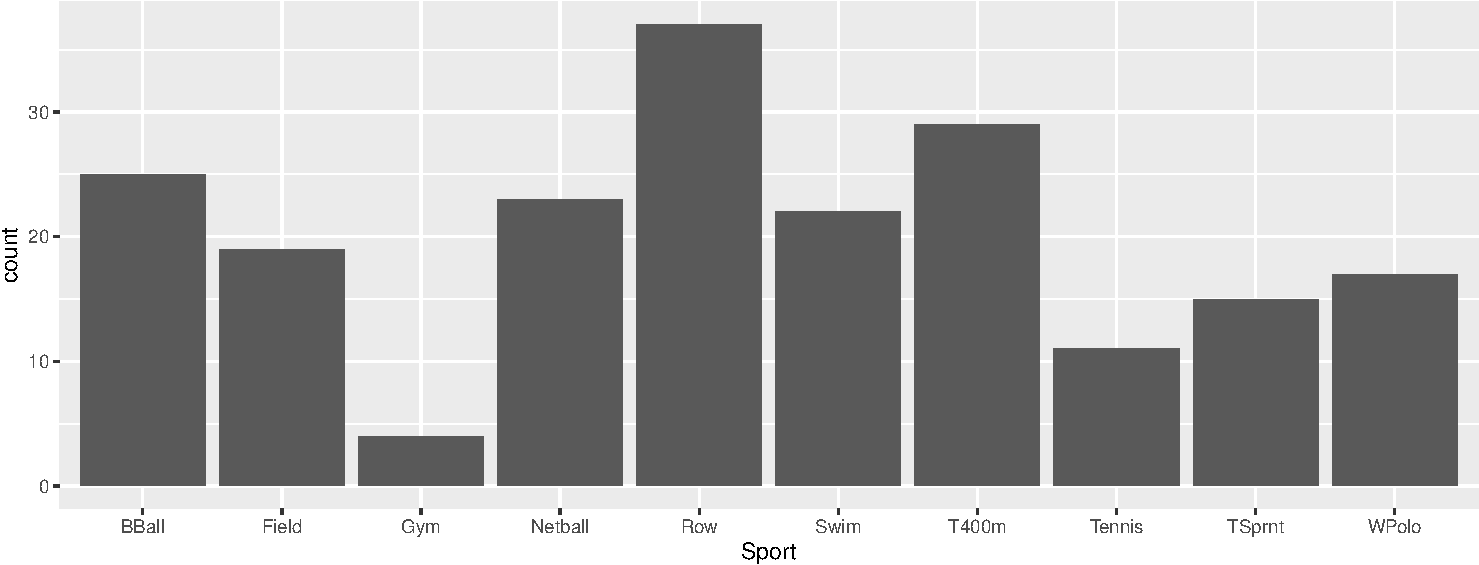
\includegraphics{graphs_files/figure-beamer/graphs-R-4-1.pdf}
\end{frame}

\begin{frame}[fragile]{Histogram of body mass index}
\phantomsection\label{histogram-of-body-mass-index}
\begin{Shaded}
\begin{Highlighting}[]
\FunctionTok{ggplot}\NormalTok{(athletes, }\FunctionTok{aes}\NormalTok{(}\AttributeTok{x =}\NormalTok{ BMI)) }\SpecialCharTok{+} \FunctionTok{geom\_histogram}\NormalTok{(}\AttributeTok{bins =} \DecValTok{16}\NormalTok{)}
\end{Highlighting}
\end{Shaded}

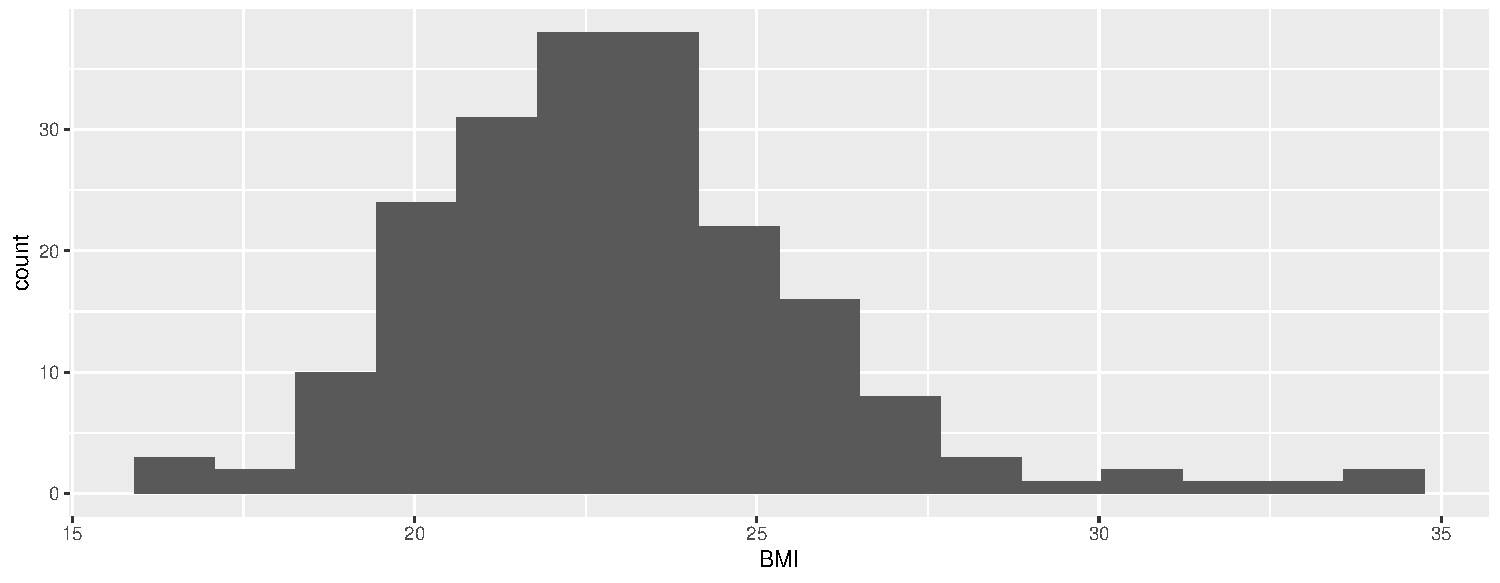
\includegraphics{graphs_files/figure-beamer/graphs-R-5-1.pdf}
\end{frame}

\begin{frame}[fragile]{Which sports are played by males and females?}
\phantomsection\label{which-sports-are-played-by-males-and-females}
Grouped bar chart:

\begin{Shaded}
\begin{Highlighting}[]
\FunctionTok{ggplot}\NormalTok{(athletes, }\FunctionTok{aes}\NormalTok{(}\AttributeTok{x =}\NormalTok{ Sport, }\AttributeTok{fill =}\NormalTok{ Sex)) }\SpecialCharTok{+}
  \FunctionTok{geom\_bar}\NormalTok{(}\AttributeTok{position =} \StringTok{"dodge"}\NormalTok{)}
\end{Highlighting}
\end{Shaded}

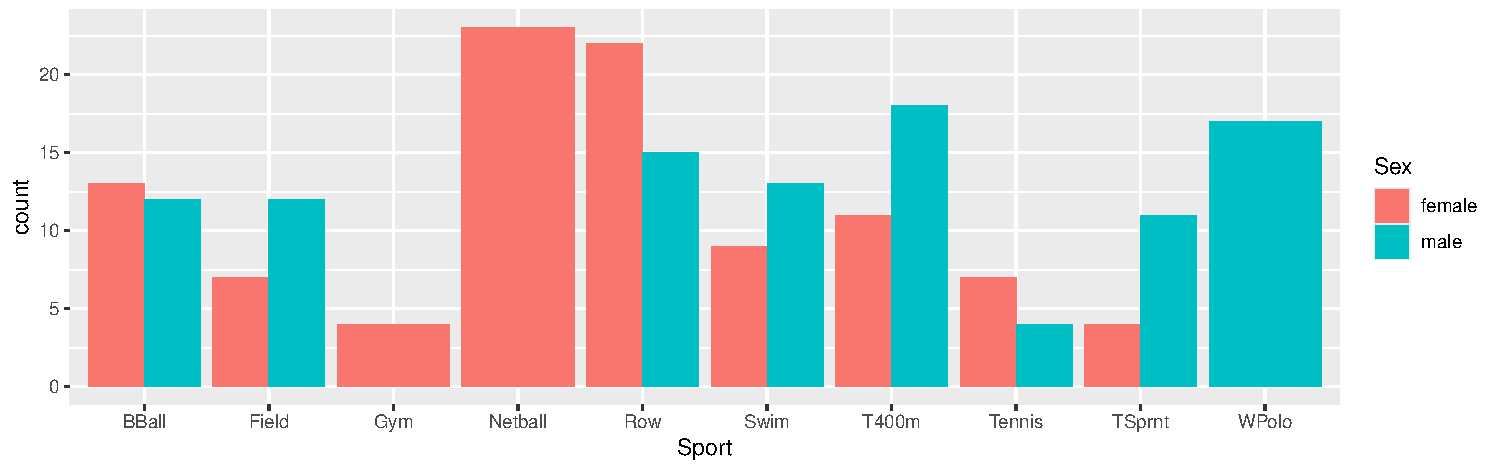
\includegraphics{graphs_files/figure-beamer/graphs-R-6-1.pdf}
\end{frame}

\begin{frame}[fragile]{BMI by gender}
\phantomsection\label{bmi-by-gender}
\begin{Shaded}
\begin{Highlighting}[]
\FunctionTok{ggplot}\NormalTok{(athletes, }\FunctionTok{aes}\NormalTok{(}\AttributeTok{x =}\NormalTok{ Sex, }\AttributeTok{y =}\NormalTok{ BMI)) }\SpecialCharTok{+} \FunctionTok{geom\_boxplot}\NormalTok{() }
\end{Highlighting}
\end{Shaded}

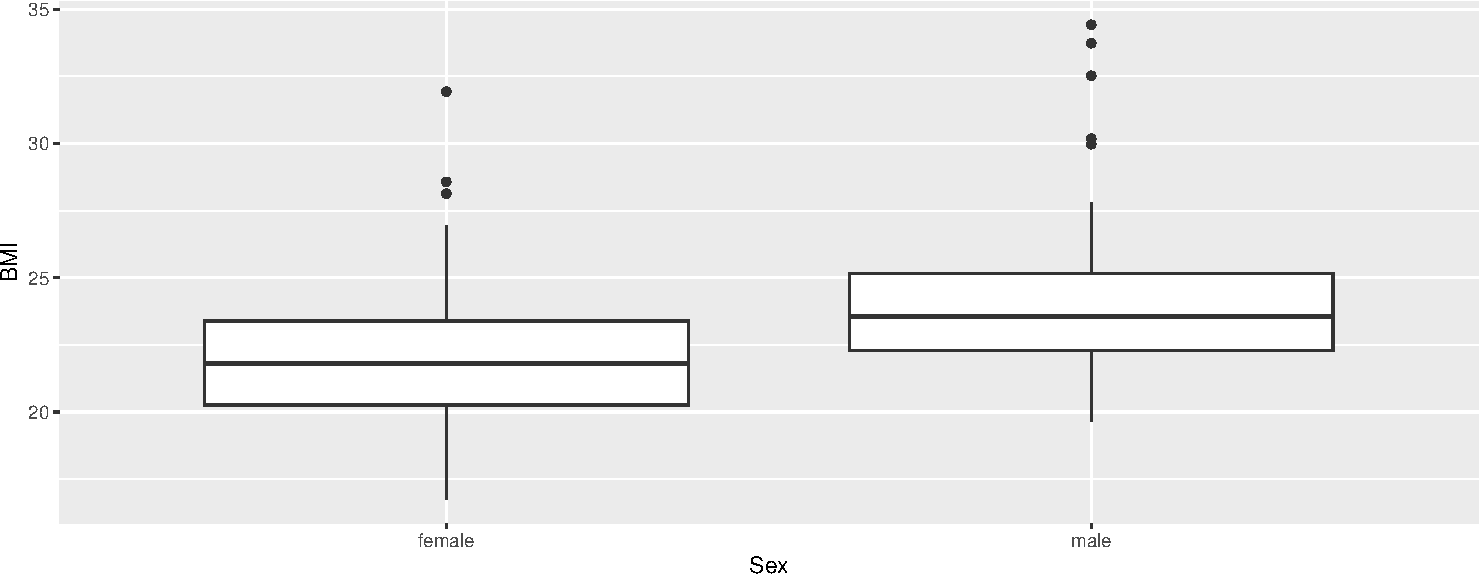
\includegraphics{graphs_files/figure-beamer/graphs-R-7-1.pdf}
\end{frame}

\begin{frame}[fragile]{Height vs.~weight}
\phantomsection\label{height-vs.-weight}
Scatterplot:

\begin{Shaded}
\begin{Highlighting}[]
\FunctionTok{ggplot}\NormalTok{(athletes, }\FunctionTok{aes}\NormalTok{(}\AttributeTok{x =}\NormalTok{ Ht, }\AttributeTok{y =}\NormalTok{ Wt)) }\SpecialCharTok{+} \FunctionTok{geom\_point}\NormalTok{()}
\end{Highlighting}
\end{Shaded}

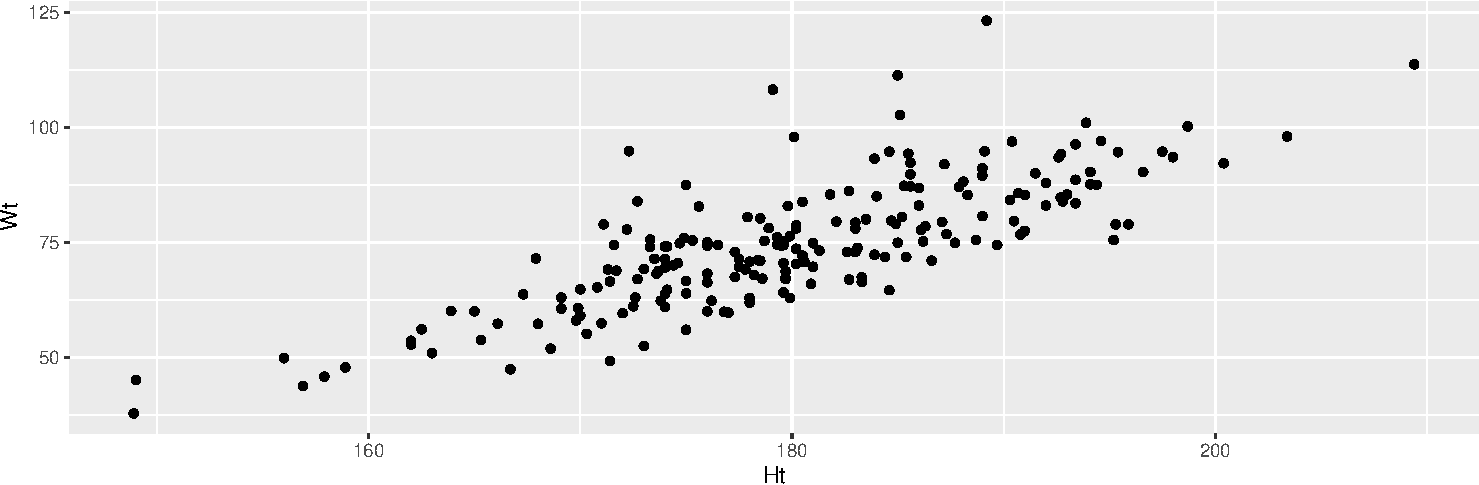
\includegraphics{graphs_files/figure-beamer/graphs-R-8-1.pdf}
\end{frame}

\begin{frame}[fragile]{With regression line}
\phantomsection\label{with-regression-line}
\begin{Shaded}
\begin{Highlighting}[]
\FunctionTok{ggplot}\NormalTok{(athletes, }\FunctionTok{aes}\NormalTok{(}\AttributeTok{x =}\NormalTok{ Ht, }\AttributeTok{y =}\NormalTok{ Wt)) }\SpecialCharTok{+}
  \FunctionTok{geom\_point}\NormalTok{() }\SpecialCharTok{+} \FunctionTok{geom\_smooth}\NormalTok{(}\AttributeTok{method =} \StringTok{"lm"}\NormalTok{)}
\end{Highlighting}
\end{Shaded}

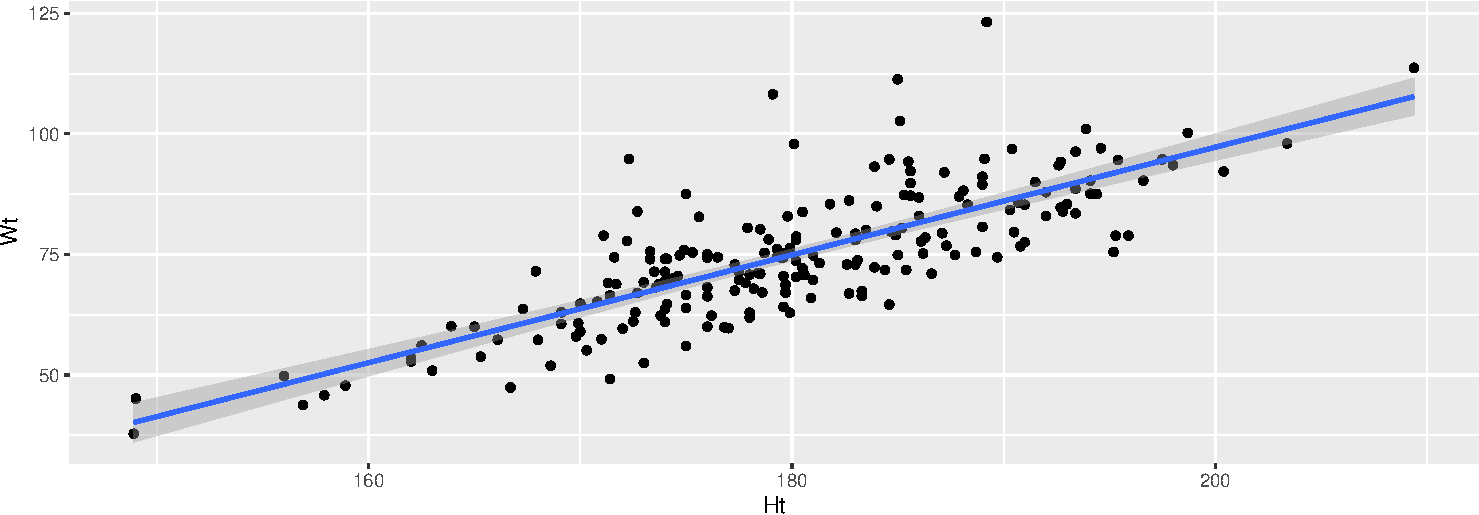
\includegraphics{graphs_files/figure-beamer/graphs-R-9-1.pdf}
\end{frame}

\begin{frame}[fragile]{BMI by sport and gender}
\phantomsection\label{bmi-by-sport-and-gender}
\begin{Shaded}
\begin{Highlighting}[]
\FunctionTok{ggplot}\NormalTok{(athletes, }\FunctionTok{aes}\NormalTok{(}\AttributeTok{x =}\NormalTok{ Sport, }\AttributeTok{y =}\NormalTok{ BMI, }\AttributeTok{fill =}\NormalTok{ Sex)) }\SpecialCharTok{+}
  \FunctionTok{geom\_boxplot}\NormalTok{()}
\end{Highlighting}
\end{Shaded}

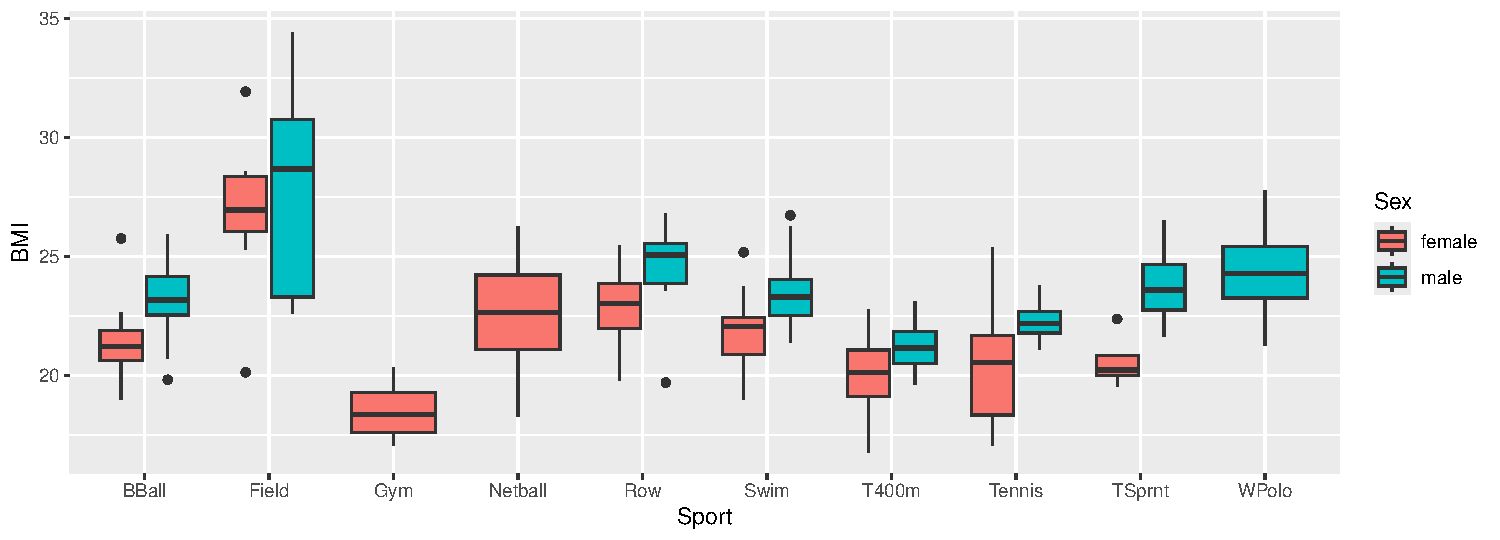
\includegraphics{graphs_files/figure-beamer/graphs-R-10-1.pdf}

A variation that uses \texttt{colour} instead of \texttt{fill}:

\begin{Shaded}
\begin{Highlighting}[]
\FunctionTok{ggplot}\NormalTok{(athletes, }\FunctionTok{aes}\NormalTok{(}\AttributeTok{x =}\NormalTok{ Sport, }\AttributeTok{y =}\NormalTok{ BMI, }\AttributeTok{colour =}\NormalTok{ Sex)) }\SpecialCharTok{+}
  \FunctionTok{geom\_boxplot}\NormalTok{()}
\end{Highlighting}
\end{Shaded}

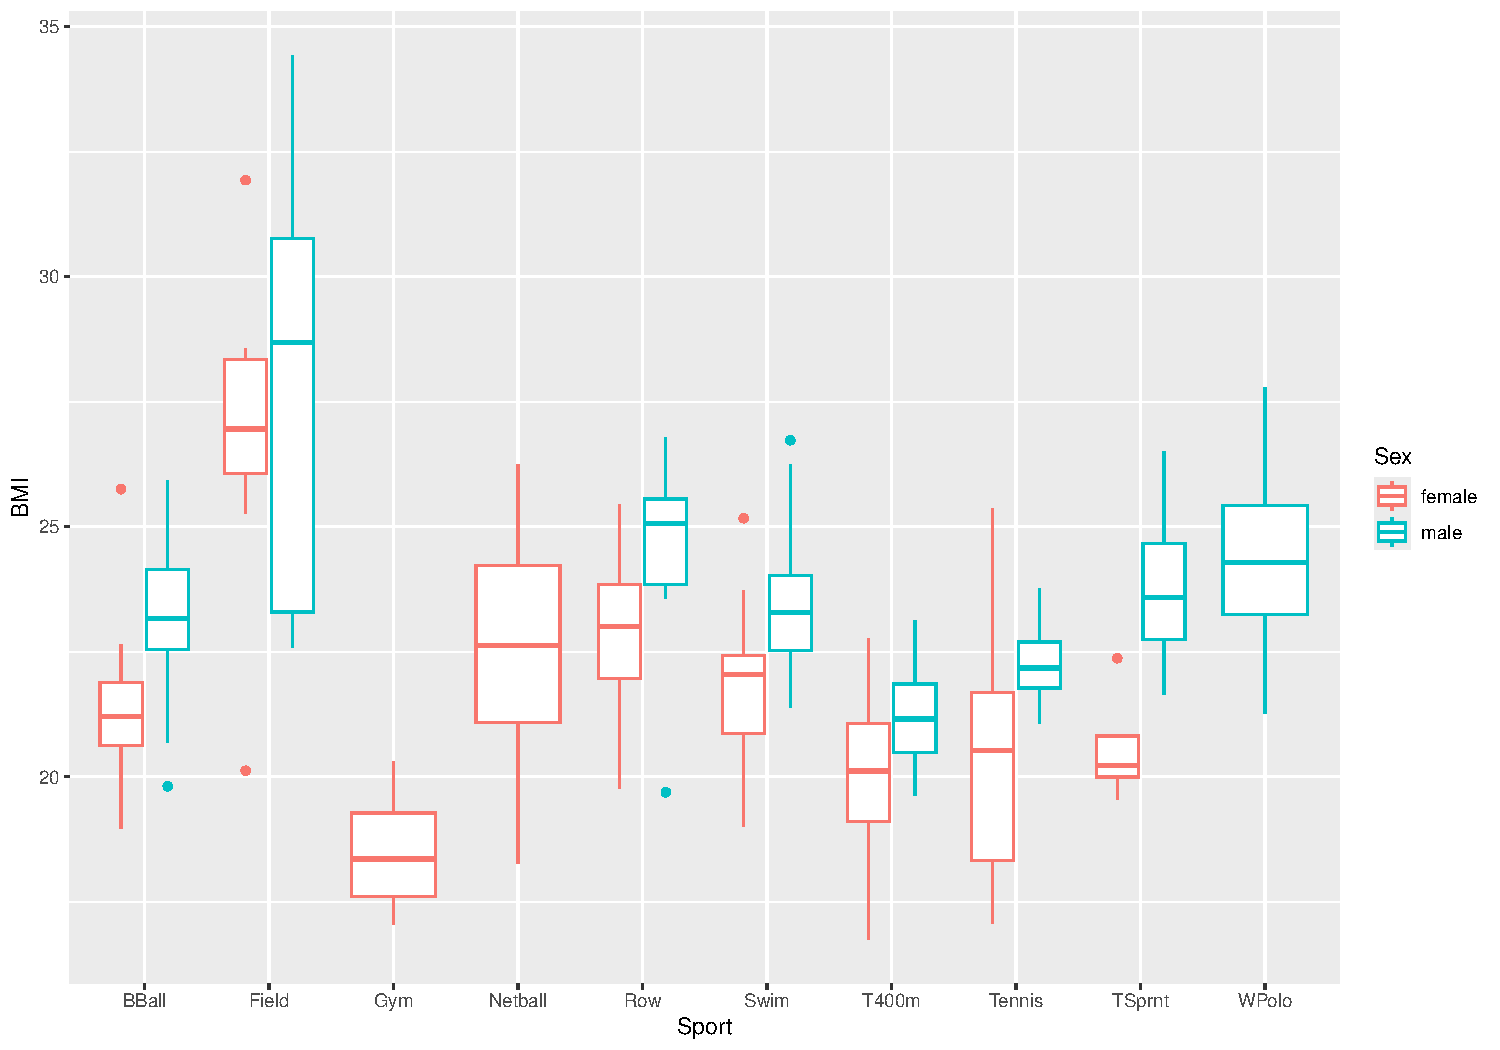
\includegraphics{graphs_files/figure-beamer/unnamed-chunk-1-1.pdf}
\end{frame}

\begin{frame}[fragile]{Height and weight by gender}
\phantomsection\label{height-and-weight-by-gender}
\begin{Shaded}
\begin{Highlighting}[]
\FunctionTok{ggplot}\NormalTok{(athletes, }\FunctionTok{aes}\NormalTok{(}\AttributeTok{x =}\NormalTok{ Ht, }\AttributeTok{y =}\NormalTok{ Wt, }\AttributeTok{colour =}\NormalTok{ Sex)) }\SpecialCharTok{+}
  \FunctionTok{geom\_point}\NormalTok{()}
\end{Highlighting}
\end{Shaded}

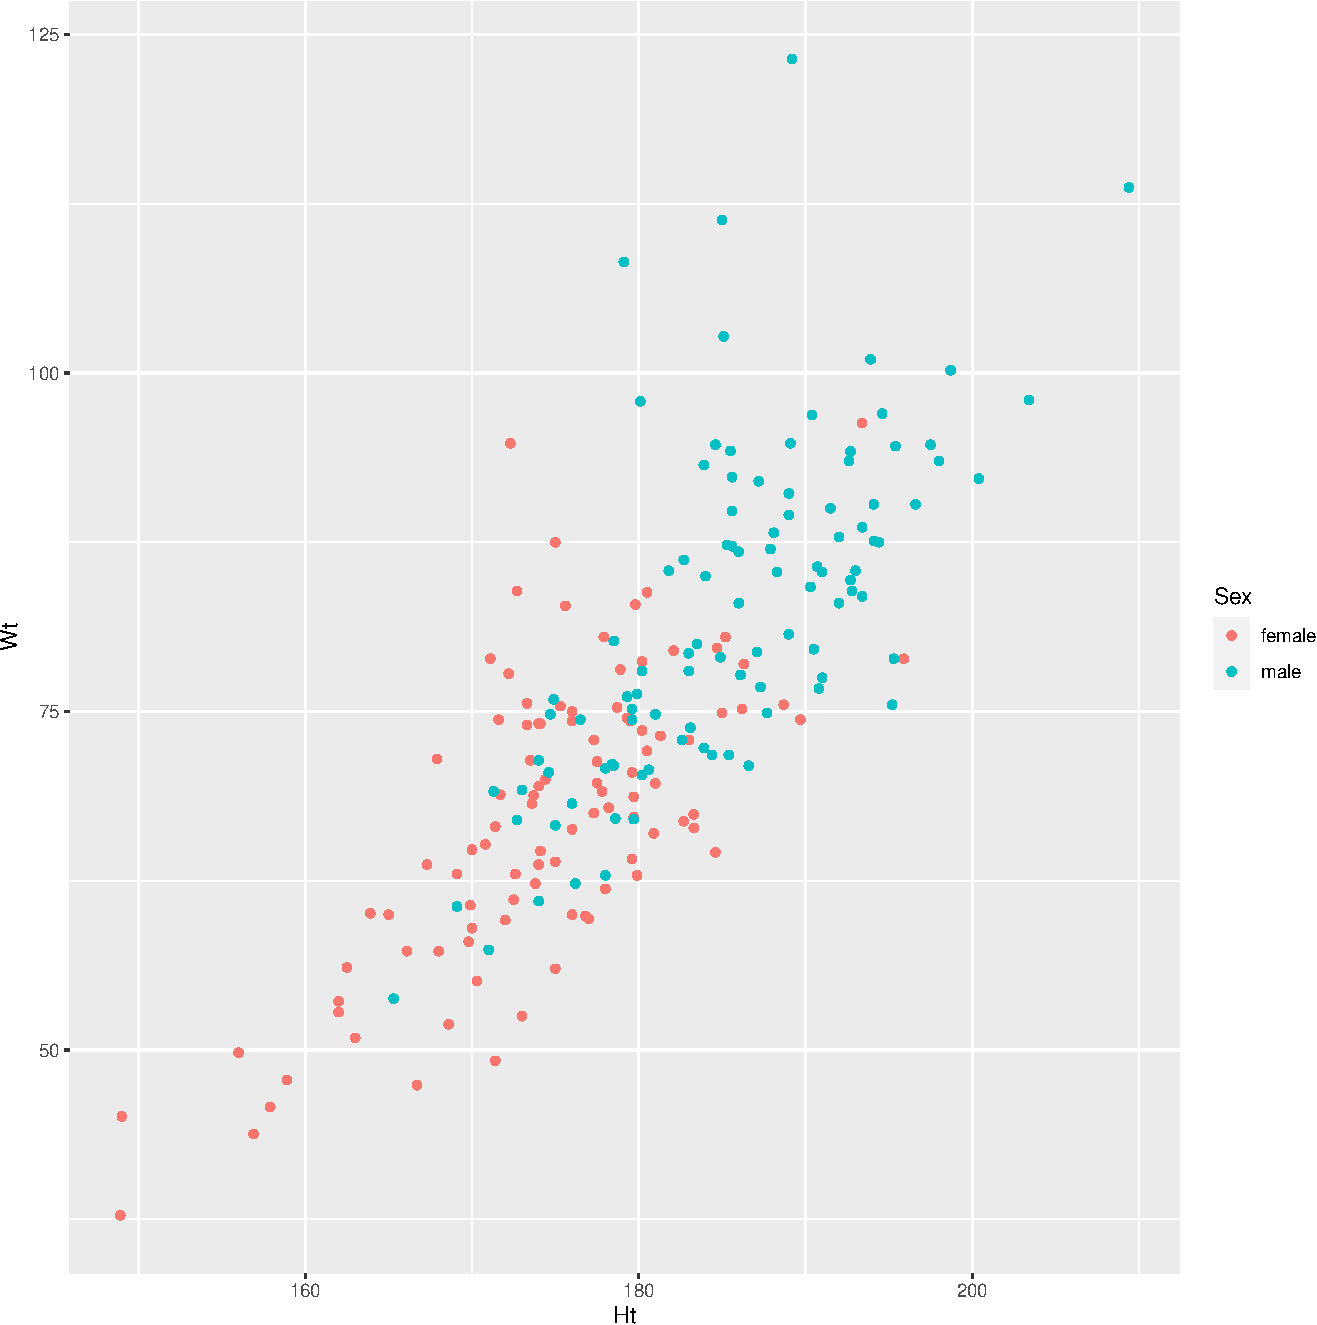
\includegraphics{graphs_files/figure-beamer/unnamed-chunk-2-1.pdf}
\end{frame}

\begin{frame}[fragile]{Height by weight by gender for each sport, with
facets}
\phantomsection\label{height-by-weight-by-gender-for-each-sport-with-facets}
\begin{Shaded}
\begin{Highlighting}[]
\FunctionTok{ggplot}\NormalTok{(athletes, }\FunctionTok{aes}\NormalTok{(}\AttributeTok{x =}\NormalTok{ Ht, }\AttributeTok{y =}\NormalTok{ Wt, }\AttributeTok{colour =}\NormalTok{ Sex)) }\SpecialCharTok{+}
  \FunctionTok{geom\_point}\NormalTok{() }\SpecialCharTok{+} \FunctionTok{facet\_wrap}\NormalTok{(}\SpecialCharTok{\textasciitilde{}}\NormalTok{Sport)}
\end{Highlighting}
\end{Shaded}

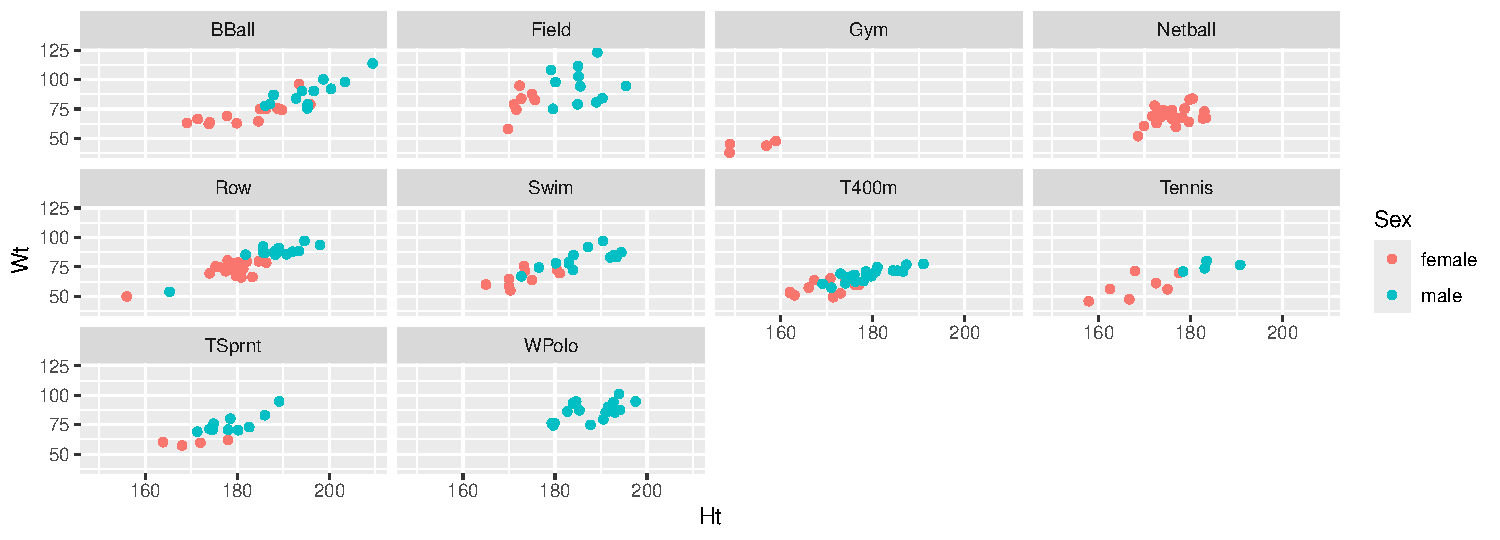
\includegraphics{graphs_files/figure-beamer/graphs-R-12-1.pdf}
\end{frame}

\begin{frame}[fragile]{Filling each facet}
\phantomsection\label{filling-each-facet}
Default uses same scale for each facet. To use different scales for each
facet, this:

\begin{Shaded}
\begin{Highlighting}[]
\FunctionTok{ggplot}\NormalTok{(athletes, }\FunctionTok{aes}\NormalTok{(}\AttributeTok{x =}\NormalTok{ Ht, }\AttributeTok{y =}\NormalTok{ Wt, }\AttributeTok{colour =}\NormalTok{ Sex)) }\SpecialCharTok{+}
  \FunctionTok{geom\_point}\NormalTok{() }\SpecialCharTok{+} \FunctionTok{facet\_wrap}\NormalTok{(}\SpecialCharTok{\textasciitilde{}}\NormalTok{Sport, }\AttributeTok{scales =} \StringTok{"free"}\NormalTok{)}
\end{Highlighting}
\end{Shaded}

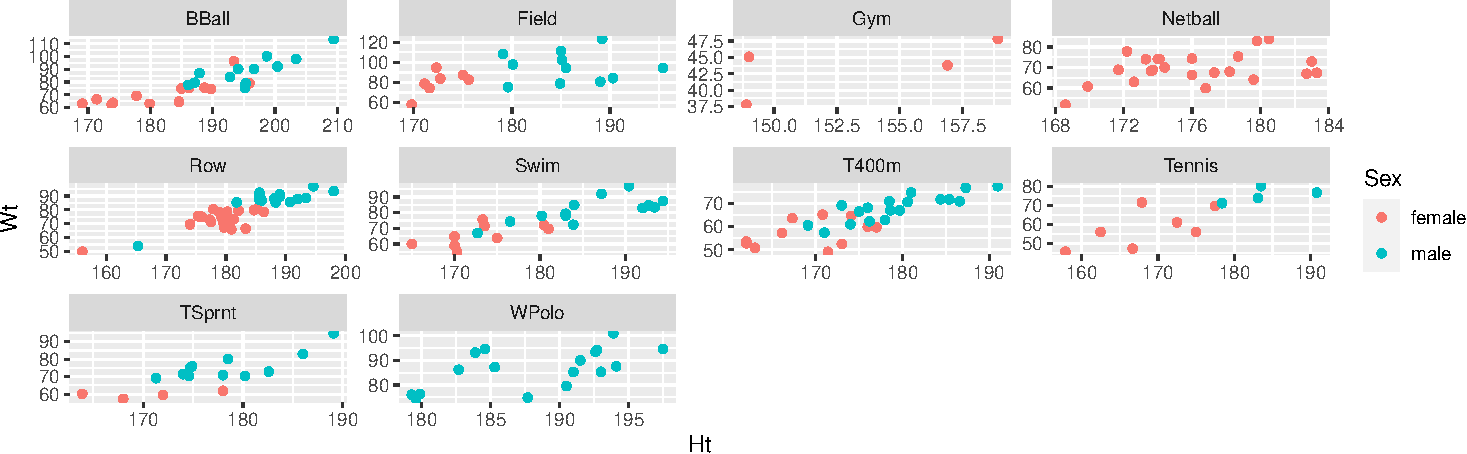
\includegraphics{graphs_files/figure-beamer/graphs-R-13-1.pdf}
\end{frame}

\begin{frame}[fragile]{Another view of height vs weight}
\phantomsection\label{another-view-of-height-vs-weight}
\begin{Shaded}
\begin{Highlighting}[]
\FunctionTok{ggplot}\NormalTok{(athletes, }\FunctionTok{aes}\NormalTok{(}\AttributeTok{x =}\NormalTok{ Ht, }\AttributeTok{y =}\NormalTok{ Wt)) }\SpecialCharTok{+}
  \FunctionTok{geom\_point}\NormalTok{() }\SpecialCharTok{+} \FunctionTok{facet\_wrap}\NormalTok{(}\SpecialCharTok{\textasciitilde{}}\NormalTok{ Sex)}
\end{Highlighting}
\end{Shaded}

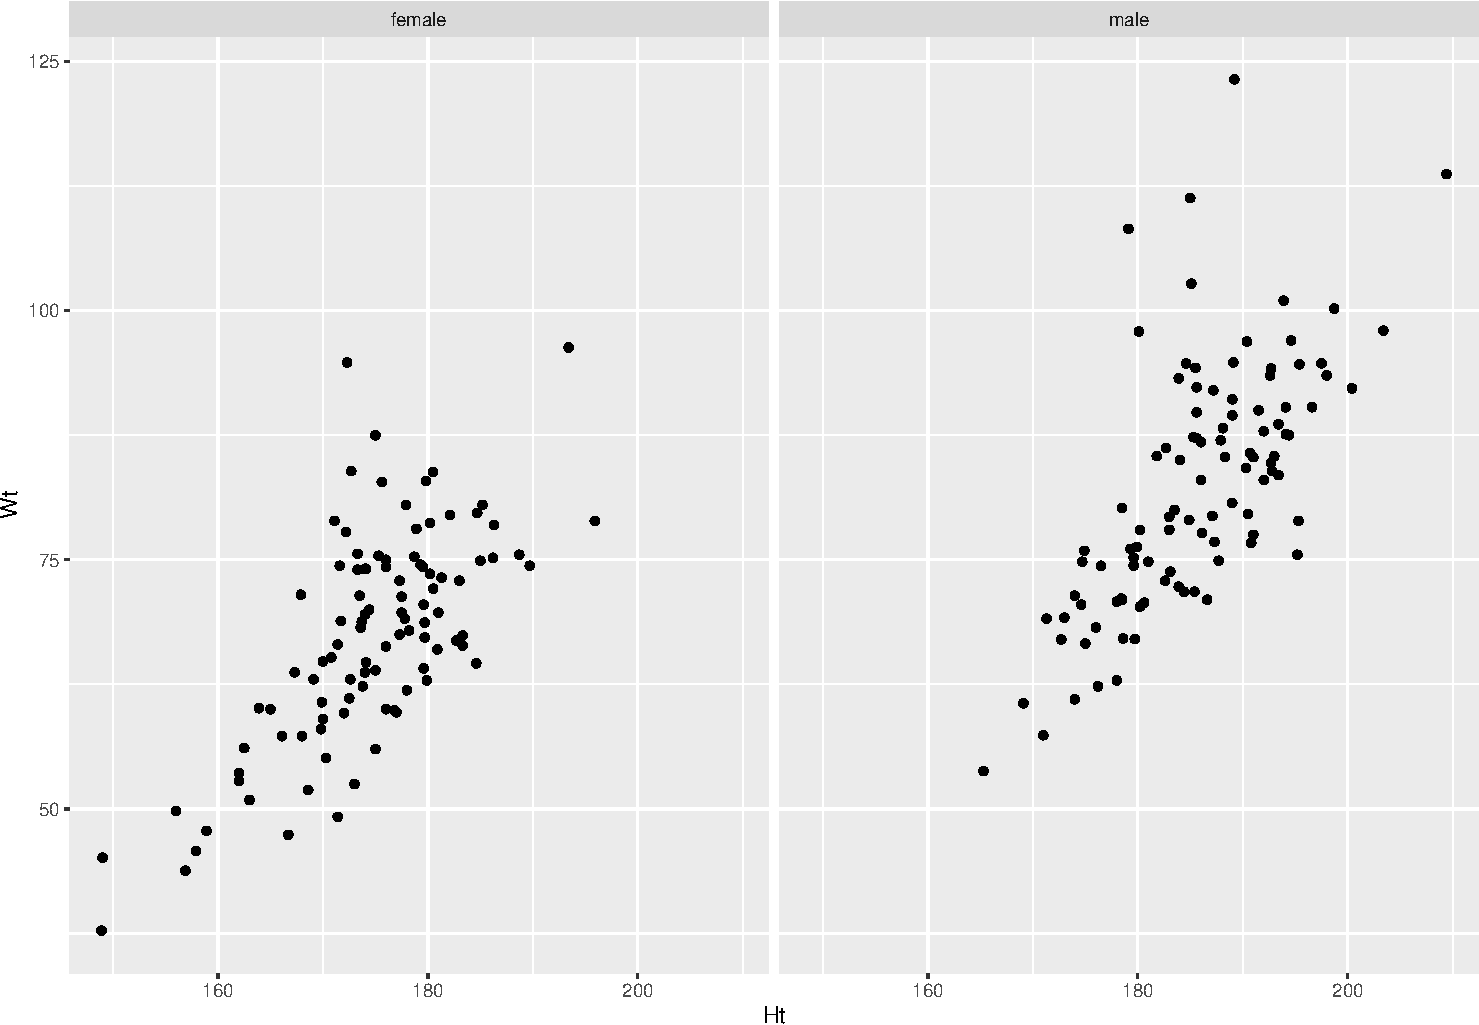
\includegraphics{graphs_files/figure-beamer/unnamed-chunk-3-1.pdf}
\end{frame}




\end{document}
